\documentclass{standalone}
\usepackage{tikz}
\usetikzlibrary{patterns, positioning}
\usepackage[sfdefault]{ClearSans} %% option 'sfdefault' activates Clear Sans as the default text font
\usepackage[T1]{fontenc}

\begin{document}
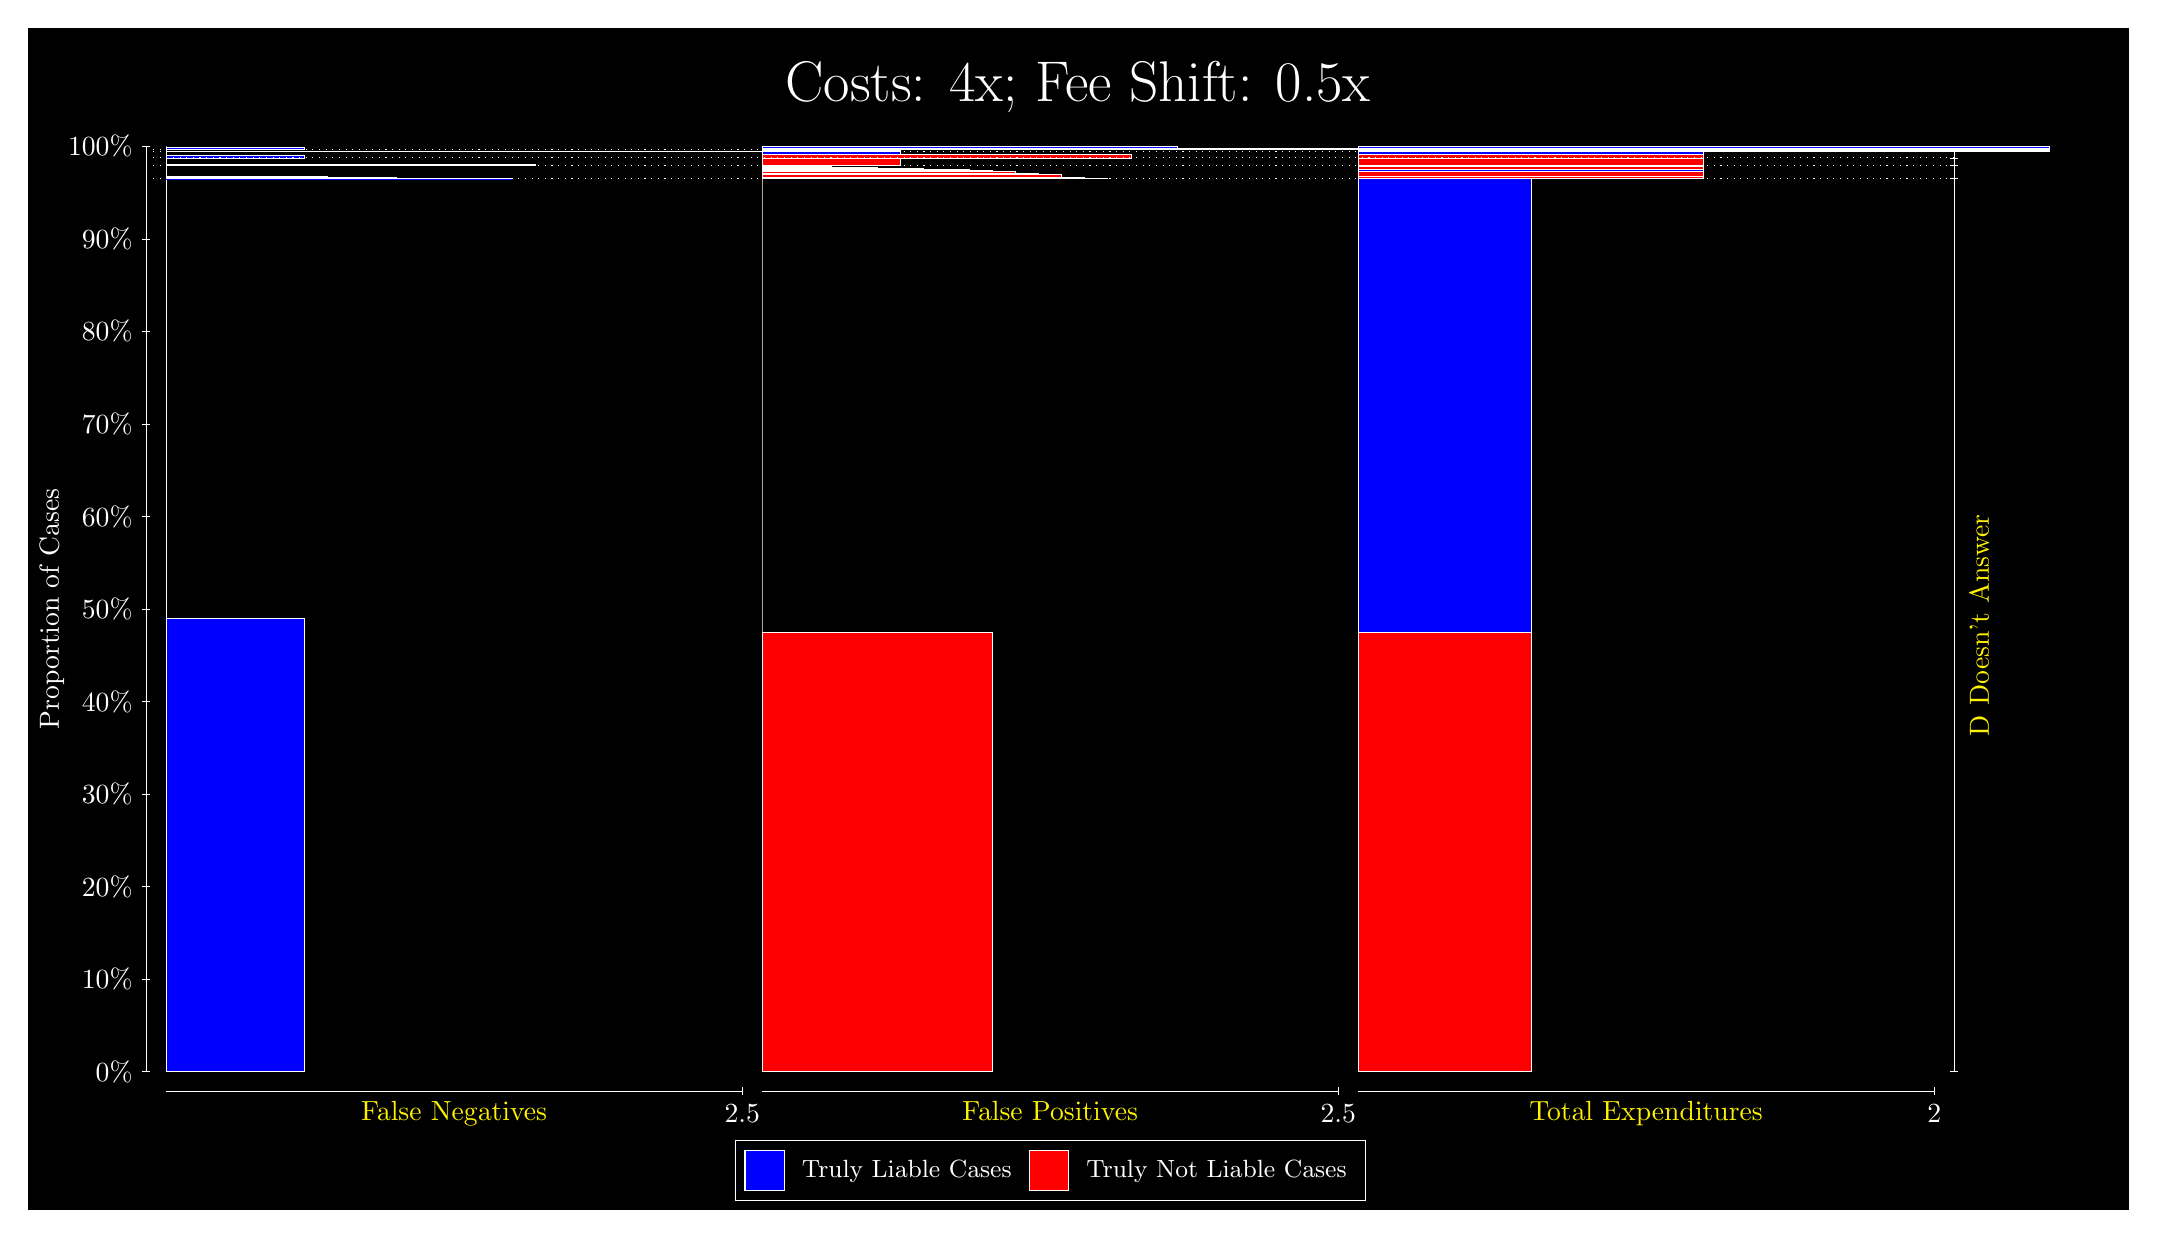
\begin{tikzpicture}
\draw[fill=black] (0,0) rectangle (26.667,15);
\draw[text=white] (0,13.5) rectangle (26.667,15) node[midway] {\huge Costs: 4x; Fee Shift: 0.5x};
\draw[white, very thin] (1.5,1.75) -- (1.5,13.5);
\node[rotate=90, text=white, anchor=center] at (0.3, 7.625) {Proportion of Cases};
\draw[white, very thin] (1.45,1.75) -- (1.55,1.75);
\node[text=white, anchor=east] at (1.45, 1.75) {0\%};
\draw[white, very thin] (1.45,2.925) -- (1.55,2.925);
\node[text=white, anchor=east] at (1.45, 2.925) {10\%};
\draw[white, very thin] (1.45,4.1) -- (1.55,4.1);
\node[text=white, anchor=east] at (1.45, 4.1) {20\%};
\draw[white, very thin] (1.45,5.275) -- (1.55,5.275);
\node[text=white, anchor=east] at (1.45, 5.275) {30\%};
\draw[white, very thin] (1.45,6.45) -- (1.55,6.45);
\node[text=white, anchor=east] at (1.45, 6.45) {40\%};
\draw[white, very thin] (1.45,7.625) -- (1.55,7.625);
\node[text=white, anchor=east] at (1.45, 7.625) {50\%};
\draw[white, very thin] (1.45,8.8) -- (1.55,8.8);
\node[text=white, anchor=east] at (1.45, 8.8) {60\%};
\draw[white, very thin] (1.45,9.975) -- (1.55,9.975);
\node[text=white, anchor=east] at (1.45, 9.975) {70\%};
\draw[white, very thin] (1.45,11.15) -- (1.55,11.15);
\node[text=white, anchor=east] at (1.45, 11.15) {80\%};
\draw[white, very thin] (1.45,12.325) -- (1.55,12.325);
\node[text=white, anchor=east] at (1.45, 12.325) {90\%};
\draw[white, very thin] (1.45,13.5) -- (1.55,13.5);
\node[text=white, anchor=east] at (1.45, 13.5) {100\%};

\draw[white, very thin] (24.457,1.75) -- (24.457,13.5);
\draw[white, very thin] (24.407,1.75) -- (24.507,1.75);
\node[anchor=west] at (24.407, 1.75) {};
\draw[white, very thin] (24.407,13.088) -- (24.507,13.088);
\node[anchor=west] at (24.407, 13.088) {};
\draw[white, very thin] (24.407,13.258) -- (24.507,13.258);
\node[anchor=west] at (24.407, 13.258) {};
\draw[white, very thin] (24.407,13.353) -- (24.507,13.353);
\node[anchor=west] at (24.407, 13.353) {};
\draw[white, very thin] (24.407,13.433) -- (24.507,13.433);
\node[anchor=west] at (24.407, 13.433) {};
\draw[white, very thin] (24.407,13.462) -- (24.507,13.462);
\node[anchor=west] at (24.407, 13.462) {};
\draw[white, very thin] (24.407,13.5) -- (24.507,13.5);
\node[anchor=west] at (24.407, 13.5) {};

\draw[white, very thin, fill=blue] (1.75,1.75) rectangle (3.5065,7.5121);
\draw[white, very thin, fill=red] (1.75,7.5121) rectangle (1.75,13.088);
\draw[white, very thin, fill=blue] (1.75,13.088) rectangle (6.1413,13.09);
\draw[white, very thin, fill=blue] (1.75,13.09) rectangle (5.8486,13.091);
\draw[white, very thin, fill=blue] (1.75,13.091) rectangle (5.5558,13.093);
\draw[white, very thin, fill=blue] (1.75,13.093) rectangle (5.2631,13.095);
\draw[white, very thin, fill=blue] (1.75,13.095) rectangle (4.9703,13.099);
\draw[white, very thin, fill=blue] (1.75,13.099) rectangle (4.6775,13.102);
\draw[white, very thin, fill=blue] (1.75,13.102) rectangle (4.3848,13.107);
\draw[white, very thin, fill=blue] (1.75,13.107) rectangle (4.092,13.11);
\draw[white, very thin, fill=blue] (1.75,13.11) rectangle (3.7993,13.121);
\draw[white, very thin, fill=red] (1.75,13.121) rectangle (1.75,13.258);
\draw[white, very thin, fill=blue] (1.75,13.258) rectangle (6.4341,13.269);
\draw[white, very thin, fill=red] (1.75,13.269) rectangle (1.75,13.353);
\draw[white, very thin, fill=blue] (1.75,13.353) rectangle (3.5065,13.385);
\draw[white, very thin, fill=red] (1.75,13.385) rectangle (1.75,13.433);
\draw[white, very thin, fill=blue] (1.75,13.433) rectangle (9.9471,13.44);
\draw[white, very thin, fill=red] (1.75,13.44) rectangle (1.75,13.462);
\draw[white, very thin, fill=blue] (1.75,13.462) rectangle (3.5065,13.492);
\draw[white, very thin, fill=red] (1.75,13.492) rectangle (1.75,13.5);
\draw[white, very thin, fill=red] (9.3189,1.75) rectangle (12.246,7.3264);
\draw[white, very thin, fill=blue] (9.3189,7.3264) rectangle (9.3189,13.088);
\draw[white, very thin, fill=red] (9.3189,13.088) rectangle (13.71,13.095);
\draw[white, very thin, fill=red] (9.3189,13.095) rectangle (13.417,13.11);
\draw[white, very thin, fill=red] (9.3189,13.11) rectangle (13.125,13.14);
\draw[white, very thin, fill=red] (9.3189,13.14) rectangle (12.832,13.161);
\draw[white, very thin, fill=red] (9.3189,13.161) rectangle (12.539,13.187);
\draw[white, very thin, fill=red] (9.3189,13.187) rectangle (12.246,13.197);
\draw[white, very thin, fill=red] (9.3189,13.197) rectangle (11.954,13.208);
\draw[white, very thin, fill=red] (9.3189,13.208) rectangle (11.661,13.214);
\draw[white, very thin, fill=red] (9.3189,13.214) rectangle (11.368,13.225);
\draw[white, very thin, fill=blue] (9.3189,13.225) rectangle (10.783,13.236);
\draw[white, very thin, fill=blue] (9.3189,13.236) rectangle (10.49,13.239);
\draw[white, very thin, fill=blue] (9.3189,13.239) rectangle (10.197,13.244);
\draw[white, very thin, fill=blue] (9.3189,13.244) rectangle (9.9044,13.247);
\draw[white, very thin, fill=blue] (9.3189,13.247) rectangle (9.6116,13.252);
\draw[white, very thin, fill=blue] (9.3189,13.252) rectangle (9.3189,13.258);
\draw[white, very thin, fill=red] (9.3189,13.258) rectangle (11.075,13.342);
\draw[white, very thin, fill=blue] (9.3189,13.342) rectangle (9.3189,13.353);
\draw[white, very thin, fill=red] (9.3189,13.353) rectangle (14.003,13.401);
\draw[white, very thin, fill=blue] (9.3189,13.401) rectangle (11.075,13.433);
\draw[white, very thin, fill=red] (9.3189,13.433) rectangle (11.075,13.455);
\draw[white, very thin, fill=blue] (9.3189,13.455) rectangle (9.3189,13.462);
\draw[white, very thin, fill=red] (9.3189,13.462) rectangle (17.516,13.47);
\draw[white, very thin, fill=blue] (9.3189,13.47) rectangle (14.588,13.5);
\draw[white, very thin, fill=red] (16.888,1.75) rectangle (19.083,7.3264);
\draw[white, very thin, fill=blue] (16.888,7.3264) rectangle (19.083,13.088);
\draw[white, very thin, fill=red] (16.888,13.088) rectangle (21.279,13.114);
\draw[white, very thin, fill=blue] (16.888,13.114) rectangle (21.279,13.118);
\draw[white, very thin, fill=red] (16.888,13.118) rectangle (21.279,13.184);
\draw[white, very thin, fill=blue] (16.888,13.184) rectangle (21.279,13.205);
\draw[white, very thin, fill=red] (16.888,13.205) rectangle (21.279,13.25);
\draw[white, very thin, fill=blue] (16.888,13.25) rectangle (21.279,13.258);
\draw[white, very thin, fill=red] (16.888,13.258) rectangle (21.279,13.342);
\draw[white, very thin, fill=blue] (16.888,13.342) rectangle (21.279,13.353);
\draw[white, very thin, fill=red] (16.888,13.353) rectangle (21.279,13.401);
\draw[white, very thin, fill=blue] (16.888,13.401) rectangle (21.279,13.433);
\draw[white, very thin, fill=red] (16.888,13.433) rectangle (25.67,13.455);
\draw[white, very thin, fill=blue] (16.888,13.455) rectangle (25.67,13.462);
\draw[white, very thin, fill=red] (16.888,13.462) rectangle (25.67,13.47);
\draw[white, very thin, fill=blue] (16.888,13.47) rectangle (25.67,13.5);
\draw[white, dotted] (1.5,13.088) -- (24.457,13.088);
\draw[white, dotted] (1.5,13.258) -- (24.457,13.258);
\draw[white, dotted] (1.5,13.353) -- (24.457,13.353);
\draw[white, dotted] (1.5,13.433) -- (24.457,13.433);
\draw[white, dotted] (1.5,13.462) -- (24.457,13.462);
\draw[white, very thin] (1.75,1.5) -- (9.0689,1.5);
\node[text=yellow, anchor=north] at (5.4094, 1.5) {False Negatives};
\draw[white, very thin] (9.0689,1.45) -- (9.0689,1.55);
\node[text=white, anchor=north] at (9.0689, 1.45) {2.5};

\draw[white, very thin] (9.3189,1.5) -- (16.638,1.5);
\node[text=yellow, anchor=north] at (12.978, 1.5) {False Positives};
\draw[white, very thin] (16.638,1.45) -- (16.638,1.55);
\node[text=white, anchor=north] at (16.638, 1.45) {2.5};

\draw[white, very thin] (16.888,1.5) -- (24.207,1.5);
\node[text=yellow, anchor=north] at (20.547, 1.5) {Total Expenditures};
\draw[white, very thin] (24.207,1.45) -- (24.207,1.55);
\node[text=white, anchor=north] at (24.207, 1.45) {2};

\node[text=yellow, centered, rotate=90] at (24.777, 7.4192) {D Doesn't Answer};






\draw (12.978300999999998,1.5) node[draw=none] (baseCoordinate) {};
\begin{scope}[align=center]
        \matrix[scale=0.5, draw=white, below=0.5cm of baseCoordinate, nodes={draw}, column sep=0.1cm]{
            \node[rectangle, draw, minimum width=0.5cm, minimum height=0.5cm, fill=blue] {}; &
            \node[draw=none, font=\small, text=white] (B) {Truly Liable Cases}; &
            \node[rectangle, draw, minimum width=0.5cm, minimum height=0.5cm, fill=red] {}; &
            \node[draw=none, font=\small, text=white] (B) {Truly Not Liable Cases}; \\
            };
\end{scope}

\end{tikzpicture}
\end{document}